\documentclass[tikz,border=0mm,convert={outfile=\jobname.png}]{standalone}
\usepackage{tikz}
\usetikzlibrary{decorations.pathmorphing,patterns}
\definecolor{spring}{HTML}{586e75}

\begin{document}

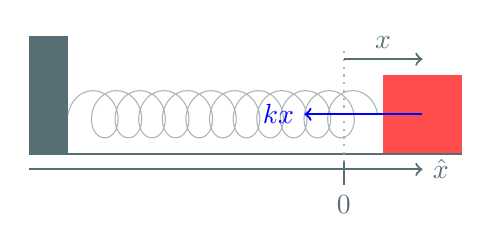
\begin{tikzpicture}
    % Draw the wall
    \fill[spring] (-0.5, 0) rectangle (0, 1.5);

    % Draw the spring
    \draw[spring!50, decorate, decoration={coil, aspect=0.8, segment length=3mm, amplitude=3mm}] (0, 0.5) -- (4, 0.5);

    % Draw the mass
    \fill[red!70] (4, 0) rectangle (5, 1);

    % Ground line
    \draw[thick,spring] (-0.5, 0) -- (5, 0);

    \draw[thick, spring, ->] (-0.5, -0.2) -- (4.5, -0.2) node[right] at (4.5, -0.2) {$\hat{x}$};
    \draw[thick, spring!50, dotted] (3.5, -0.4) -- (3.5, 1.3);
    \draw[thick, spring, ->] (3.5, 1.2) -- (4.5, 1.2) node[above] at (4, 1.2) {$x$};
    \draw[thick, blue, ->] (4.5, 0.5) -- (3, 0.5) node[left] at (3, 0.5) {$kx$};
    \draw[thick, spring] (3.5, -0.1) -- (3.5, -0.4) node[below] at (3.5, -0.4) {$0$};
\end{tikzpicture}

\end{document}

%%% Local Variables:
%%% mode: LaTeX
%%% TeX-master: t
%%% End:
